\section{Durchführung}
Das Sagnac-Interferometer wird, wie in Abbildung $\ref{aufbau}$ dargestellt, aufgebaut. Als Lichtquelle wird ein Helium-Neon-Laser genutzt, da dieser die, für die Interferenzeffekte nötige, Kohärenz des Lichts stellt.
Vor dem PBSC wird außerdem ein Polarisationsfilter angebracht, welcher unter anderem für die Kontrastbestimmung benötigt wird. Damit die in der Theorie bereits beschriebene Funktionsweise gewährleistet ist,
ist es notwendig das Interferometer mit Hilfe von Beam-Paddles zu justieren und eine optische Achse einzustellen. Ziel hierbei ist zunächst dafür zu sorgen, dass die Teilstrahlen sich überlagern. Als Justiermöglichkeiten
stehen hierbei Drehregler an den Spiegeln, Metallplättchen unter den Bauelementen und ein gewisser Freiraum an der Befestigung des PBSCs zur Verfügung. Es ist außerdem darauf zu achten, dass die Teilstrahlen
nach dem Austreten aus dem zweiten PBSC die Öffnungen der Photodioden treffen.
\begin{figure}[H]
  \centering
  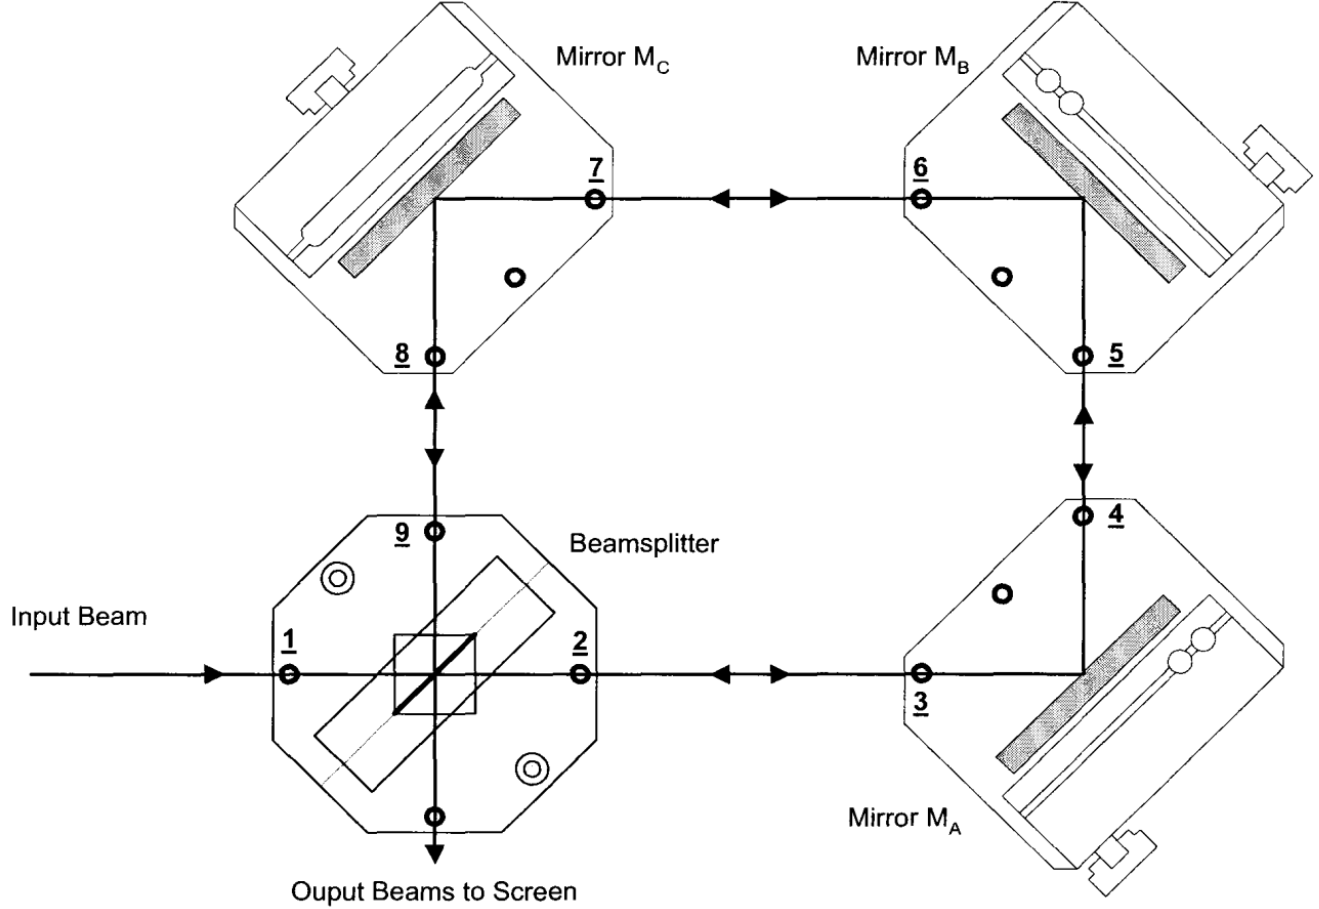
\includegraphics[scale=0.4]{Bilder/skizze2.png}
  \caption{Schematische Darstellung des Versuchsaufbaus.\cite{anleitung}}
  \label{aufbau}
\end{figure}
Wenn das Interferometer vollständig justiert ist, kann die Kontrastbestimmung beginnen. Hierzu wird zunächst der Polarisationsfilter auf $0°$ gestellt, die angewinkelten Glasplättchen in dem Interferometer platziert
und die beiden Teilstrahlen durch Spiegel leicht versetzt.
Es werden die Intensitätsmaxima und -minima aufgezeichnet. Für jeden Messwert wird zunächst ein Polarisationswinkel eingestellt, dann wird der Winkel der Glasplättchen variiert und die so entstehenden
Intensitätsschwankungen über ein, mit der Photodiode verbundenes, Oszilloskop notiert.
\subsection{Brechungsindexbestimmung}
Für die Brechungsindexbestimmung wird das Interferometer auf den Maximalkontrast eingestellt. Für Glas werden die bereits bei der Kontrastbestimmung genutzten Glasplättchen verwendet.
Mit einen dem Versuch zugehörigen Counter, lässt sich aus der Differenz der Signale an den Photodioden, die Anzahl der Interferenzmaxima bestimmen. Es wird sechs Mal über eine Spanne von $10°$ der Winkel der Glasplättchen
variiert und dabei die Anzahl der Interferenzmaxima aufgezeichnet.\\
Zur Untersuchung des Brechungsindexes von Luft wird anstelle der Glasplättchen eine Gaskammer angebracht. Diese wird über eine Pumpe auf wenige $\si{\milli\bar}$ abgepumpt. Die so evakuierte Gaszelle lässt sich
über Ventile kontrolliert belüften. Es wird mindestens drei Mal die evakuierte Zelle auf Normaldruck belüftet und dabei die Anzahl der Interferenzmaxima notiert.
